\documentclass[../main.tex]{subfiles}
\graphicspath{{\subfix{../images/}}}

\begin{document}
\begin{enumerate}
    \item We have that \[m=\tan{\theta}, \frac{dm}{dx}=\sec^2{\theta}\frac{d\theta}{dx}.\]
Substituting into the above equation, we get:
\begin{align*}
    (D-x)\frac{dm}{dx}=\lambda\sqrt{1+m^2} &\Longrightarrow (D-x)\sec^2{\theta}\frac{d\theta}{dx}=\lambda\sec{\theta} \\
    &\Longrightarrow \int \sec{\theta}\,d\theta = \int \frac{\lambda}{D-x}\,dx && D-x > 0\\
    &\Longrightarrow \ln\left(\sec{\theta}+\tan{\theta}\right)=-\lambda\ln{(D-x)}+C' &&m>0 \Longrightarrow 0 < \theta < \frac{\pi}{2}\\
    &\Longrightarrow \sec{\theta}+\tan{\theta}=C(D-x)^{-\lambda} \\
    &\Longrightarrow m+\sqrt{1+m^2}=C(D-x)^{-\lambda}
\end{align*}
Finally, applying the initial conditions gives
$$m+\sqrt{1+m^2}=\left(\frac{D-x}{D}\right)^{-\lambda}=\left(1-\frac{x}{D}\right)^{-\lambda}.$$
\item While we are tempted to directly apply $\frac{d}{dx}(Vt)=\sqrt{1+m^2}$, this is most likely difficult to simplify given that we now have an expression in $Vt$. No good. It may be wiser to use the result for $\frac{dm}{dx}$, so that
\begin{align*}
    m+\sqrt{1+m^2}=\left(1-\frac{x}{D}\right)^{-\lambda} &\Longrightarrow m+\frac{D-x}{\lambda}\frac{dm}{dx}=\left(1-\frac{x}{D}\right)^{-\lambda}\\
    &\Longrightarrow \frac{dm}{dx}+\frac{\lambda}{D-x}m=\frac{\lambda}{D-x}\left(1-\frac{x}{D}\right)^{-\lambda}=\lambda D^{\lambda}(D-x)^{-\lambda-1}
\end{align*}
Now we proceed by the integrating factor approach, where the integrating factor is simply $(D-x)^{-\lambda}$:
Thus,
\begin{align*}
    m(D-x)^{-\lambda}&=\int \lambda D^{\lambda}(D-x)^{-2\lambda-1} \,dx \\
    &= \frac{D^{\lambda}(D-x)^{-2\lambda}}{2}+C \\
    m &= \frac{D^{\lambda}(D-x)^{-\lambda}}{2}+C(D-x)^{\lambda}
\end{align*}
Applying the initial conditions gives $$m=\frac{dy}{dx}=\frac{D^{\lambda}(D-x)^{-\lambda}}{2}-\frac{(D-x)^{\lambda}}{2D^{\lambda}}.$$

Finally, back-integrating gives $$y=\frac{D^{\lambda}(D-x)^{-\lambda+1}}{2(\lambda-1)}+\frac{(D-x)^{\lambda+1}}{2D^{\lambda}(\lambda+1)}+E.$$
Again, applying the initial conditions gives 
$$y=\frac{D^{\lambda}(D-x)^{-\lambda+1}}{2(\lambda-1)}+\frac{(D-x)^{\lambda+1}}{2D^{\lambda}(\lambda+1)}+\frac{D}{2(1-\lambda)}-\frac{D}{2(\lambda+1)}.$$

Indeed, we should be satisfied with this answer, because for $x \to D$, $y$ tends to the vertical line $y=\frac{D}{2(1-\lambda)}-\frac{D}{2(\lambda+1)}$. Moreover, $\frac{D}{2(1-\lambda)}-\frac{D}{2(\lambda+1)}$ is positive. If you have anxiety, a quick sketch using a graphing calculator should convince you:
\begin{figure}[H]
    \centering
    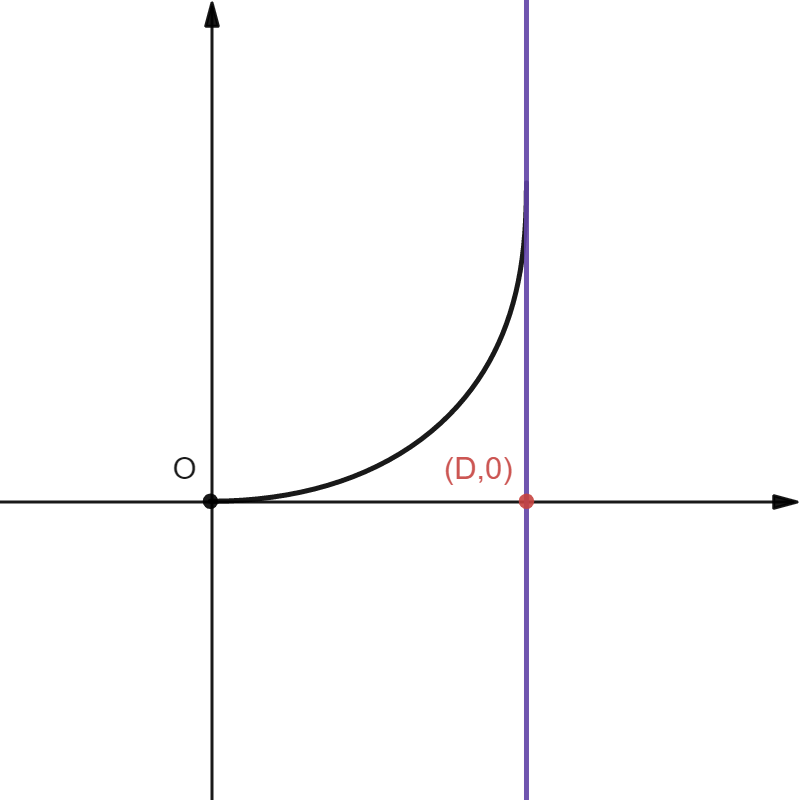
\includegraphics[scale=0.25]{graph-pursuit-sol.PNG}
    \caption{The pursuit curve for $\lambda=0.63, D=7$ (don't ask why I chose these values).}
    \label{fig:graph-pursuit-sol}
\end{figure}
\end{enumerate}

\paragraph{Solution 5.12}
The first inequality follows from the claim that $\cos{x} \leq e^{-\frac{x^2}{2}} \Longleftrightarrow f(x)=\ln{\cos{x}} \leq -\frac{x^2}{2}$ for $|x|<\frac{\pi}{2}$. This is true because $f(x)$ is:
\begin{enumerate}
    \item An even function with $f(0)=0$, and
    \item concave since $f''(x)=-\tan^2{x} < 0$.
\end{enumerate}
The second inequality follows by symmetry(!), and the last equality follows from the normal distribution $N(\mu, \sigma^2)$:
$$\frac{1}{\sigma\sqrt{2\pi}}\int_{-\infty}^{\infty}e^{-\frac{(x-\mu)^2}{2\sigma^2}} \,dx = 1$$ for the choice $\mu = 0$, $ \sigma=\frac{1}{\sqrt{2n}}$.

\end{document}